% Cap�tulo 2
\chapter{The Problem - Breakdown}\label{theProblemChap}

TODO: In this section we detail ...

\section{Problem Breakdown}
TODO: Breakdown each step of the problem.

\section{Proposed solution}

In this work we propose a set of steps to guide the transition from relational databases to NoSQL ones. The suggested guidelines make use of Service Level Agreements (SLAs) to guide the whole process. These guidelines are represented on Figure~\ref{fig:guidelinesNoSQL}.


\begin{figure}[ht!]
\centering
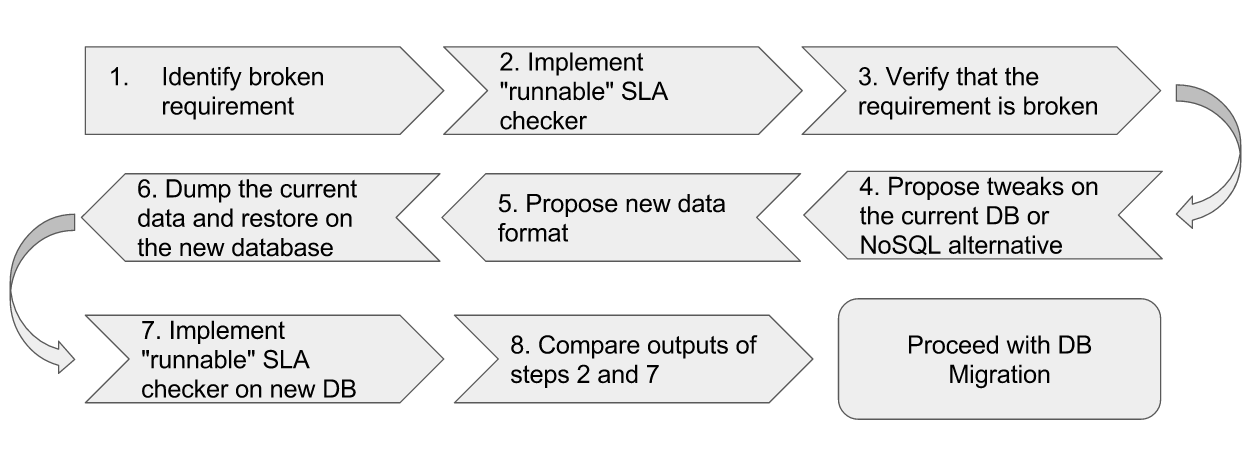
\includegraphics[width=150mm]{guidelines.png}
\caption{Relational to NoSQL Steps.\label{fig:guidelinesNoSQL}}
\end{figure}

The guidelines consist on a total of 9 steps, as follows:


\begin{enumerate}
   \item{\textbf{Identify broken requirement} - A database migration is generally motivated by performance issues. The first step in a transition scenario is to identify what are the operations or application requirements that are motivating the database transition. This can an existing requirement of the application or a new one.

   In the context of a retail business intelligence application, a possible requirement could be \textit{``I want to have a word cloud from the Twitter Bio of the customers that bought products X, Y or Z. I'd like to wait up to 5 seconds to see this word cloud.''.}}
   \item{\textbf{Implement runnable SLA checker} - On this step a runnable SLA is implemented to assure that the current DB infrastructure does not support the requirement. }
   \item{\textbf{Verify that the requirement is broken} - After having the runnable SLA implemented, it is possible to check that the requirement is not being fulfilled by the current DB infrastructure.}
   \item{\textbf{Propose modifications on the current DB or NoSQL alternative} - Not always it is necessary to change the database to address a performance problem. SQL tunning, denormalizing tables and creating indexes are popular ways to improve the performance of applications that use relational databases.

   
   Another option to address performance problems on relational databeses would be to scale-up the current DB, buying more powerful hardware. This option is not covered by this work, as budget is always a finite resource on companies.


   If the SLA remains broken after the architectural changes have been performed on the current DB infrastructure, a NoSQL strategy might be recommended. In this case, a new Database Model (Graph DBs, Document Stores, Key-value stores, etc.) and technology (Neo4j, MongoDB, Couchbase) should be chosen. 
   }

   \item{\textbf{Propose new data format} - After choosing the new NoSQL database, it is necessary to map the table elements and relations into the concepts of the chosen NoSQL technology. }
   \item{\textbf{Dump the current data and restore on the new database} - To compare the performance of RDBMS vs NoSQL on a specific scenario, the same amount of data must be present on both DBs. So, a Dump \& Restore procedure is needed on the side of the NoSQL DBs.}
   \item{\textbf{Implement runnable SLA checker on new DB} - Once the new DB is populated with production data, a new runnable SLA is needed to compare the results of the proposed architecture and the old architecture}.
   \item{\textbf{Compare outputs of steps 2 and 7} - If the new DB architecture fills the gaps of the broken requirements \textit{and other requirements are not broken with the new architecture}, the DB transition should continue.}
   \item{\textbf{Proceed with DB migration} - On this step, the source code of the application should be updated to match the new Database Architecture. }
\end{enumerate}

% % Casos a serem considerados em trabalhos futuros: 
% % > Load Tests
% % > Mapear todos os requisitos / opera��es da aplica��o na nova arquitetura.


% Esqueleto do framework/guidelines

% 1 - Criacao de SLA para cada operacao disponibilizada pelo component: Nesse passo definimos um SLA que tal servico deve obedecer (chamadas a tal endpoint devem retornar em <2s, por ex. Esse SLA servira para ``provar'' que a minha tecnologia + infraestrutura atual nao me atende satisfatoriamente.
% 2 - Criacao de um SLA (suite de testes automatizados ou qualquer coisa definida no SLA@SOI) que mostre que a aplicacao nao respeita o SLA acordado no passo anterior.
% 3 - Proposicao de nova infraestrutura/tecnologia
% 4 - Implementacao e Simulacao
% 6 - Comparacao dos testes antigos e novos
% 7 - Validacao da melhoria e cumprimento do SLA acordado na etapa 01.
% 8 - Monitoramento continuo das operacoes apos a migracao (SLA ativo)

% - A validacao do framework e da app a partir de aplicacoes de exemplo;
% - Open-source app que escuta todas as requisicoes a um servidor (JS-based e server based) e analisa se um SLA foi respeitado apos alguma mudanca;
% - Implementacao com alguma coisa de Open Stack;


\section{Roadmap}

To provide a better understanding of our work, we splitted the research in six main phases:

\begin{table}[!htb]
   \textsf{\caption{Work Phases.}} \label{tab:WorkPhasesTable}
   \centering
   \medskip
      \begin{tabular}{ | p{1cm}| p{2.5cm} | p {8cm} |}
   \hline
   Phase & Title & Description  \\ \hline
   1 & Identification of Case Studies \& SLAs  & On this step we aim to identify examples where a Database transition is needed or recommended in order to satisfy a SLA.
   We will try to work on production-ready and open-source softwares. If the complexity of these projects is too large for our scope, we will design and develop our own scenarios. \\ \hline
   2 & Plan & After the scenarios have been identified, we will propose architectural changes that could satisfy the SLA. These changes will be proposed by literature reviews and survey of industry experts.\\ \hline
   3 & Do & On this step we implement the architecture proposed on the previous step. \\ \hline
   4 & Check & On the check step we will verify if the proposed architecture and implementation satisfies the SLAs identified on the first step. \\ \hline
   5 & Act & Tweaks can be needed on the proposed architecture and implementation if the SLA is still not satisfied by the changes made on the previous step. On the act phase we investigate what else can be done to satisfy the SLA and refine the process defined on step 2. \\ \hline
   6 & Final Results & On the final step we aim to publish the results of our work on relevant database-related conferences and workshops. \\ \hline
   
   \end{tabular}
\end{table}





Each of these phases is composed by a number of steps, described below:
\begin{enumerate}
\item{Phase 1 - Identification of Case Studies \& SLAs }
\begin{enumerate}
\item {Step 1.1 - Scenario identification / Implementation: On this step we will search for open source projects and real-world scenarios where a Relational Database bottleneck has been identified. If the scope of these scenarios become too large, we will implement our own scenarios; }
\item {Step 1.2 - Identification of broken SLAs: We need to identify that the a set a constraints (i.e: execution time of a query) is not being met by the current architecture;}
\item {Step 1.3 - Implementation of ``runnable SLAs'' : On this step we will implement executable versions of the SLA identified on the previous step. These ``runnable SLAs" will be used to verify that a set of constraints is not being met by the current architecture. }
\item {Step 1.4 - Execution reports: After an executable SLA has been identified and implemented, execution reports will be consolidated to prove that the constraints of the SLA are being broken by the current architecture of the scenario.}

\end{enumerate}


\item{Phase 2 - Plan}
\begin{enumerate}
\item{Step 2.1 - Literature Review for each scenario: We will evaluate and search for solutions on how each scenario can make use of a NoSQL Database to meet the desired SLA; }
\item{Step 2.2 - Survey of industry experts: We will survey industry experts on how they would propose a NoSQL architecture to solve the problem described on each scenario. }
\end{enumerate}

\item{Phase 3 - Do}
\begin{enumerate}
\item{Step 3.1 - Planning of changes: We will gather the results from the previous phase and design the changes that will be performed on each scenario;}
\item{Step 3.2 - Implementation: We will implement the changes identified on the previous step. }
\end{enumerate}

\item{Phase 4 - Check}
\begin{enumerate}
\item {Step 4.1 - New Execution Reports: The same SLAs identified on the first step will be run on the modified scenarios, and execution reports will be consolidated.}
\item {Step 4.2 - Comparison of Results: The reports extracted on steps 4.1 and 1.4 will be compared to check if the changes made on Phase 3 satisfied the proposed SLA.}
\end{enumerate}

\item{Phase 5 - Act}
\begin{enumerate}
\item{Step 5.1 - Tweaks on the proposed architecture: If the SLA isn't being met yet, new changes might be needed, and on this step we join together the phases 2, 3 and 4 to iterate over the needed changes. }
\end{enumerate}


\item{Phase 6 - Final Results}
\begin{enumerate}
\item{Step 6.1 - Publish the results: We will submit the results of this study to academical conferences to have feedback from the community. }
\item{Step 6.2 - Write the final results: All the documents produced by our study and a final dissertation will be sent to the Universidade Federal do Rio Grande do Norte (UFRN).}


\section{Schedule}

A detailed view of the execution flow of our steps can be seen on Figure~\ref{fig:schedule}. 
\begin{figure}[ht!]
\centering
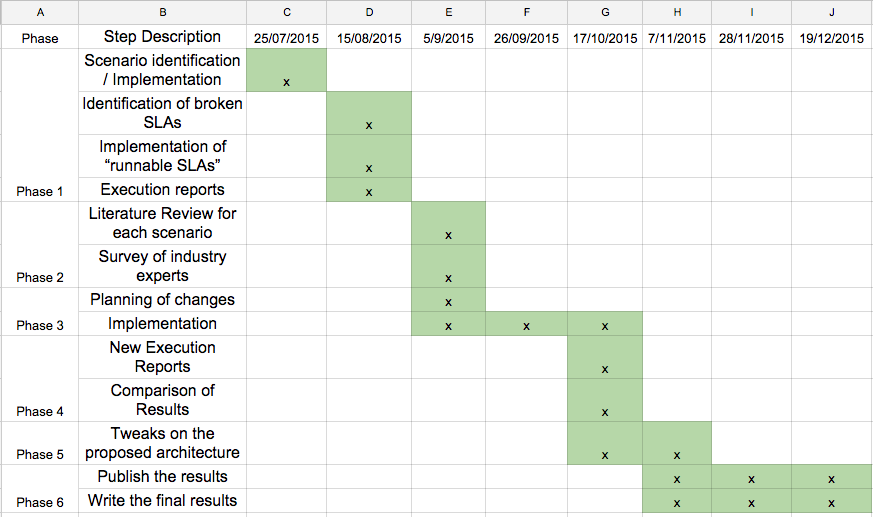
\includegraphics[width=140mm]{schedule.png}
\caption{Schedule.\label{fig:schedule}}
\end{figure}
\end{enumerate}

\end{enumerate}
